\documentclass[10pt,a4paper]{article}
\usepackage[utf8]{inputenc}
\usepackage[english]{babel}
\usepackage[T1]{fontenc}
\usepackage{amsmath}
\usepackage{amsfonts}
\usepackage{amssymb}
\usepackage{amsthm}
\usepackage{dsfont}

\usepackage{hyperref}
\usepackage{cite}


\usepackage{graphicx}

\theoremstyle{definition}
\newtheorem{definition}{Definition}
\theoremstyle{definition}
\newtheorem{theorem}{Theorem}
\theoremstyle{definition}
\newtheorem{notation}{Notation}

\author{Della Bona Sarah, Dumez Erika}
\title{Introduction to Neural ODE}
\begin{document}
\maketitle

\newpage
\tableofcontents

\newpage
\section{Introduction}

In this document, we introduce ODE-nets, which are deep neural networks models using ordinary differential equations. We focus in particular on the mathematical aspects of these neural networks. We will give definitions and properties for different notions such as ordinary differential equations, regular and residual neural networks, implicit layers, ... 

\noindent At the end, we'll conclude with the advantages and disadvantages of ODE-nets.
The code use to make the examples can be found at \url{https://github.com/DumezErika/ProjetMachineLearning}.


\section{Ordinary Differential Equations}

An\textit{ ordinary differential equation} (ODE) \cite{9} is an equation that describes the changes of a function through time. The aim is to compute that function from the ODE which describes its derivative. In this setting, time is a continuous variable.

\begin{definition}
Let $\Omega \subseteq \mathbb{R} \times \mathbb{R}^N$ an open set. Let $f: \Omega \rightarrow \mathbb{R}^N$. 

A \textit{first order ODE} takes the form
$$
\frac{\partial u}{\partial t}(t) = f(t,u(t))
$$

\begin{itemize}
\item A \textit{solution} for this ODE is a function $u : I\in \mathbb{R} \rightarrow \mathbb{R}^N$, where $I$ is an interval, such that
	\begin{itemize}
	\item[•] u is differentiable on $I$,
	\item[•] $\forall t \in I, (t, u(t)) \in \Omega$,
	\item[•] $\forall t \in I, \frac{\partial u}{\partial t}(t) = f(t, u(t))$
	\end{itemize}
~

\item An \textit{initial condition} (IC) is a condition of the type
$$
u(t_0) = u_0
$$
where $(t_0, u_0) \in \Omega$ is fixed.

~

\item A \textit{Cauchy problem} is an ODE with IC
$$
\left \{
\begin{array}{rcl}
\frac{\partial u}{\partial t}(t) & = & f(t, u(t)) \\
u(t_0) & = & u_0
\end{array}
\right.
$$
\end{itemize}
\end{definition}

%\begin{definition}
%A \textit{k-order ODE}, with $k \in \mathbb{N}\backslash \{0\}$, takes the form
%$$
%\partial^k_t v(t) = g(t, v(t), ... , \partial^{k-1}v(t))
%$$
%where 
%
%\begin{align*}
%v &:  I \rightarrow \mathbb{R}^N, I\subset \mathbb{R} \\ 
%g &:  \Theta \subseteq \mathbb{R} \times \mathbb{R}^N \times ... \times \mathbb{R}^N \rightarrow \mathbb{R}^N
%\end{align*} 
%\end{definition}

\subsection{A simple example}
Let $\frac{\partial x}{\partial t}(t) = x(t)$ an ODE. The solutions of this ODE are
$$
\{ x(t) = ae^t\ |\ a\in \mathbb{R}\}.
$$

Indeed, for all $a \in \mathbb{R}$ we have
$$
\frac{\partial ae^t}{\partial t} = ae^t
$$
If we add an initial condition $x(0) = 1$, we have a Cauchy problem and its solution is $e^t$, since $e^0 = 1$ and $\partial_te^t = e^t$.

\subsection{Existence and uniqueness of a solution} \label{exiunique}

If we want to find the solution to an ODE, we need to know the conditions under which this ODE has a solution. Thus, we define \textit{Lipschitz continuous functions}. This notion is crucial for the following theorem which gives conditions for the existence and uniqueness of a solution to an ODE.

\begin{definition}
Let $(X, d_X)$ and $(Y, d_Y)$ be two metric spaces.  
A function 

\noindent $f: X \rightarrow  Y$ is called \textit{Lipschitz continuous} if
$$
\exists K \geq 0, \  \forall x_1, x_2 \in X, \  d_Y(f(x_1), f(x_2)) \leq Kd_X(x_1, x_2).
$$
\end{definition}

\begin{theorem}{\textbf{Picard-Lindelöf theorem}}

Consider the Cauchy problem
$$
\frac{\partial u}{\partial t} (t) = f(t, u(t)), \ \ \ u(t_0) = u_0.
$$
Suppose $f$ is uniformly Lipschitz continuous in $u$ and continuous in $t$. Then for some value $T > 0$, there exists a unique solution $u(t)$ to the Cauchy problem on the interval $[t_0, t_0 + T]$. 
\end{theorem}

\subsection{One-step methods}
Unfortunately, it is not always possible to explicitly find a solution to a Cauchy problem. However, let $T > 0$ such that the solution $u$ exists on $[t_0, t_0 + T]$ and let $n \geqslant 2$ be a natural. Let  $t_0 < ... < t_n \in [t_0, t_0 + T]$ where $t_n = t_0 + T$. We can compute a finite number of points $(u_1, \dots, u_n)$ such that:
$$
\forall i\in \{0,\dots, n\},  u_i \approx u(t_i).
$$

To compute those points, we use \textit{one-step methods} which compute the points $u_{i+1}$ from the previous point $u_i$, the time $t_i$ and the \textit{step} $h_i := t_{i+1} - t_i$.

\subsection{Euler's method} \label{euler}
Euler's method is a one-step method with a constant step $h$. It is similar to a Taylor development (q.v. Section \ref{annex}), the idea is to compute $u(t_{i+1})$ using the formula
\begin{equation}\label{eqeuler}
u(t_{i+1}) \approx u(t_i) + h\frac{\partial u}{\partial t}(t_i)
\end{equation}
where 
$$
\frac{\partial u}{\partial t}(t_i) = f(t_i, u(t_i)).
$$


\section{Neural Networks}
In a typical machine learning problem \cite{10}, we have an output variable $Y$ to $p$ predictors $X_1,\dots, X_p$, also called input variable, where $p\in \mathbb{N}\backslash \{0\}$. The inputs belongs to an input space $\mathcal{X}$ and usually $\mathcal{X} \subset \mathbb{R}^p$. The output belongs to a output space $\mathcal{Y}$. It depends on the problem, for example: if this is a regression problem, $\mathcal{Y} \subset \mathbb{R}$. But if we have a classification problem with $K$ categories, $\mathcal{Y} = \{1,2,\dots, K\}$.

Let's assume that there is some relationship between $Y$ and $X = (X_1,\dots, X_p)$, which can be written in the general form
$$
Y = f(X) + \epsilon.
$$
Here $f$ is some fixed but unknown function, called \textit{target function}, of $X_1, \dots, X_p$ and $\epsilon$ is a random error term which is independent of $X$ and has mean zero and finite variance.

The goal of machine learning is to estimate this function $f$ as precisely as possible. To do that, we need a \textit{data set} to learn. The data is a set of $n$ points in $\mathcal{X} \times \mathcal{Y}$
$$
\mathcal{D} = \{(x_1, y_1),\dots, (x_n,y_n)\}.
$$

Let $x$ be a data point, then we can predict its output $y$ using 
$$
\hat{y} = \hat{f}(x),
$$
where $\hat{f}$ represents our estimate for $f$, and $\hat{y}$ represents the resulting prediction for $y$.

To determine the precision of an estimation $\hat{f}$, we use a \textit{loss function}, which is a function of a prediction and the output given by the target function. Some example of loss functions are
\begin{itemize}
\item Square error loss: $\mathcal{L}(y, \hat{y}) = (y-\hat{y})^2$;
\item Absolute error loss: $\mathcal{L}(y, \hat{y}) = |y - \hat{y}|$;
\item Zero-one loss: $\mathcal{L}(y, \hat{y}) = \mathds{1}_{\{(y, \hat{y}) | y\neq \hat{y}\}}(y, \hat{y})$.
\end{itemize}


\subsection{Definition}


\noindent A \textit{neural network} \cite{8} can be used to solve a machine learning problem. It consists of a series of layers. There are three types of layers :

\begin{itemize}
\item The \textit{input} layer
\item The \textit{output} layer
\item The \textit{hidden} layers
\end{itemize}

Each layer consist of a certain number of neurons. We give an input $x$ to the neurons of a layer, they do some calculus and give an output $z$. An \textit{activation function} is then applied to this output and obtain a value $h$ before transmitting it to the next layer thanks to the connections between the neurons of each layer. The simplest example of a neural network layer is 

$$
h = \sigma (wx +b)
$$
where $\sigma$ is an activation function, $w$ is a weight matrix and $b$ a bias vector.

~

%TODO mettre les formules directement dans la définition
We begin by giving an input to the input layer, which transmits information to the first hidden layer\footnote{There isn't always an hidden layer in a neural network}. In turn, it transmit information to the next layer and so on, until the output layer gives us the final output, the \textit{prediction}. An example of neural network is given in figure \ref{examplenn}.

\begin{figure}
\center
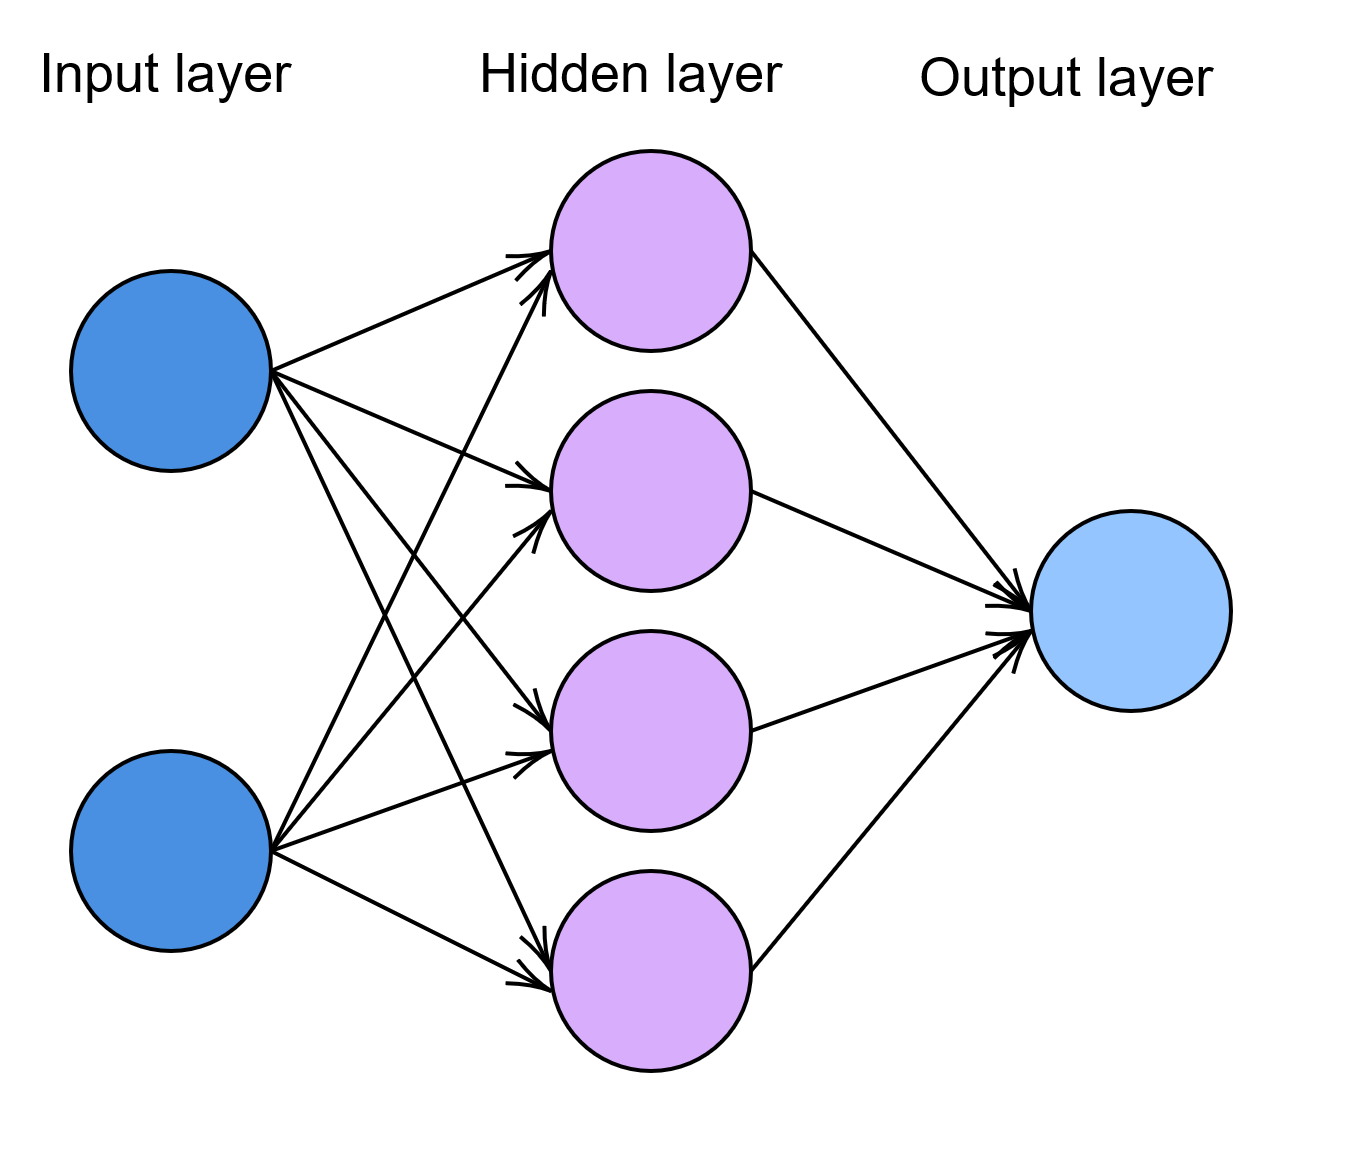
\includegraphics[scale=0.2]{nn.png}
\caption{Example of neural network}
\label{examplenn}
\end{figure}

The goal is to minimize the error for every input. To do that, we need to find the optimal parameters for the network which minimize the loss function.



\subsection{Back propagation}
Let $\theta$ be the parameters of the network. We want to find $\theta$ which minimize the loss function in order to have the error as small as possible. Therefore, we need to determine the partial derivative of the loss function with respect to the parameters, $\frac{\partial L}{\partial \theta}$. Indeed, we know that if the partial derivative of a function is $0$ at a certain point, then this point is a local extremum. 

Backpropagation \cite{11} is the process used to compute this derivative. It works by computing the gradient of the loss function with respect to each parameter by the chain rule, computing the gradient one layer at a time, iterating backward from the final layer to avoid redundant calculations of intermediate terms in the chain rule.

\subsection{Example} \label{exnn}
Let's consider a neural network with one hidden layer that takes a two-dimensional input $x = (x_1, x_2)$ and gives a 2-dimensional output $\hat{y} = (\hat{y_1},\hat{y_2})$. We can represent this network with the following equations:

\begin{eqnarray*}
z & = & w^{(1)}x + b^{(1)} \\ 
h & = & \sigma (z)\\
\hat{y} & = &  w^{(2)}h + b^{(2)} \\
\mathcal{L} & = & \frac{1}{2} \| \hat{y} - y \|_2^2
\end{eqnarray*}
   
where $w^{(1)}, w^{(2)} \in \mathbb{R}^2\times \mathbb{R}^2$ and $b^{(1)}, b^{(2)} \in \mathbb{R}^2$ are parameters of the network.

We can now use the backpropagation algorithm to easily compute $\frac{\partial \mathcal{L}}{\partial w^{(1)}}, \frac{\partial \mathcal{L}}{\partial w^{(2)}},\frac{\partial \mathcal{L}}{\partial b^{(1)}},\frac{\partial \mathcal{L}}{\partial b^{(2)}}$, the partial derivatives of the loss function with regards to the parameters.

\begin{figure}
\center
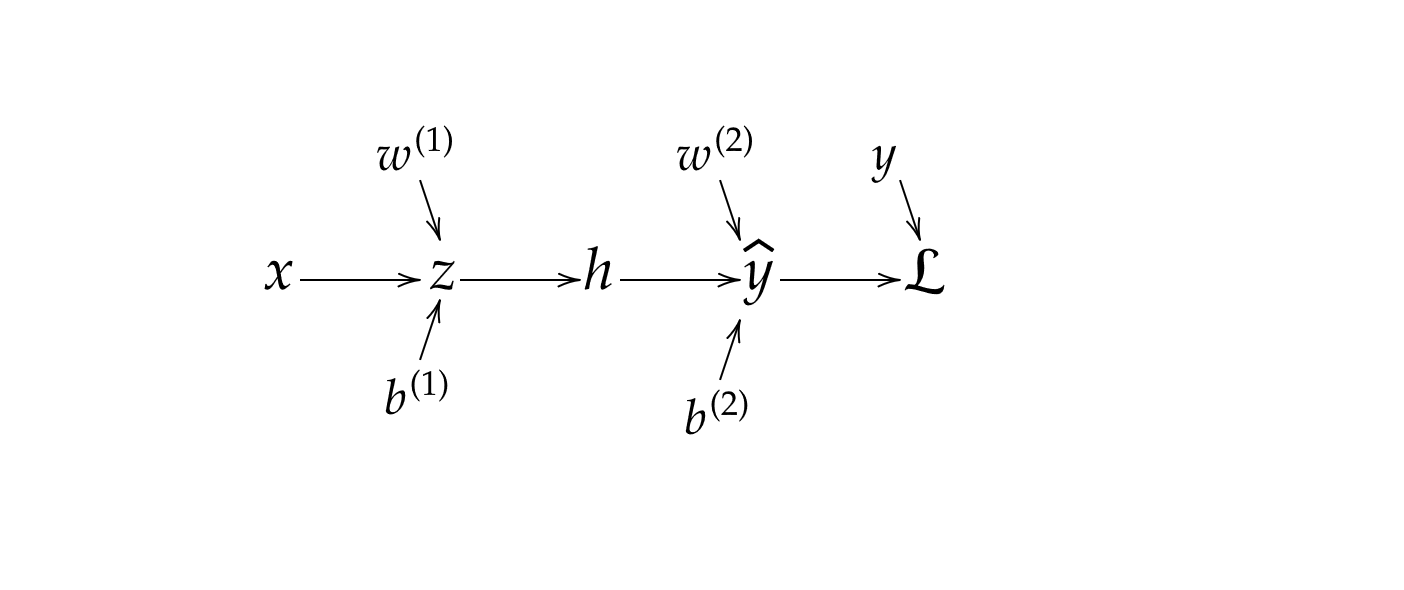
\includegraphics[scale=0.5]{computation_graph.png}
\caption{Computation graph}
\end{figure}

\begin{eqnarray*}
\frac{\partial \mathcal{L}}{\partial \mathcal{L}} & = & 1 \\
\frac{\partial \mathcal{L}}{\partial \hat{y}} & = & \frac{\partial \mathcal{L}}{\partial \mathcal{L}} \ (\hat{y} - y) \\
\frac{\partial \mathcal{L}}{\partial w^{(2)}} & = & \frac{\partial \mathcal{L}}{\partial \hat{y}}\ h^T \\
\frac{\partial \mathcal{L}}{\partial b^{(2)}} & = & \frac{\partial \mathcal{L}}{\partial \hat{y}} \\
\frac{\partial \mathcal{L}}{\partial h} & = &  (w^{(2)})^T\ \frac{\partial \mathcal{L}}{\partial \hat{y}} \\
\frac{\partial \mathcal{L}}{\partial z} & = & \frac{\partial \mathcal{L}}{\partial h} \circ \sigma '(z) \\
\frac{\partial \mathcal{L}}{\partial w^{(1)}} & = & \frac{\partial \mathcal{L}}{\partial z}\ x^T \\
\frac{\partial \mathcal{L}}{\partial b^{(1)}} & = & \frac{\partial \mathcal{L}}{\partial z} \\
\end{eqnarray*}

\subsection{Gradient descent}

\textit{Gradient descent} \cite{10} is a process used to find a local minimum of a differentiable function. It works as follow: at each step of the process, we take a step in the opposite direction of the gradient of the function at the current point, because this is the direction of the steepest descent.

More formally, if we have a function $f: \mathbb{R}^n \rightarrow \mathbb{R}$, $n>1$, differentiable and a point $x_0\in \mathbb{R}^n$, we have that if
$$
x_{n+1} = x_n -\gamma_n \nabla f(x_n), n\geq 0
$$
for $\gamma_n \in \mathbb{R}^+$ small enough, then $f(x_n) \geq f(x_{n+1})$. 

We get a sequence $x_0,x_1,\dots$ that converges to the desired local minimum under some conditions (q.v. Annex: theorem \ref{thmconvgd}), such that
$$
f(x_0) \geq f(x_1) \geq \dots . 
$$

If the function $f$ is convex, all local minima are also global minima, so the gradient descent can converge to the global minimum.

\subsection{Vanishing and exploding gradient}

The problem when using the gradient descent algorithm on neural network is that each weight is updated using the partial derivative of the loss function with regards to the current weight, and if this gradient is too small, it will prevent the weight from changing its value. In this case, the neural network will not be able to learn.

One example of this problem is when we use the hyperbolic tangent as activation function. Because this function has gradients in the range $]0,1[$ and backpropagation computes gradients by the chain rule, we multiply several of these small numbers which leads the gradient to decrease exponentially. The deeper is the neural network, the more likely this problem can occur.

The exploding gradient problem is the opposite, it happens when the derivatives take on larger values.

%TODO regarder à comment expliquer formellement, peut-être un exemple et des dessins? 

\subsection{Residual neural network} \label{rnn}

A\textit{ residual neural network} \cite{6}, also called ResNet, is simply a regular neural network except that it has more connections. Not only do we feed the output of the previous layer to the next, but also the input of that layer. 
An example of the representation of a ResNet is given in Figure \ref{exampleresnet}.

In these networks, the output of the $k+1$th layer is given by
\begin{equation*}
x_{k+1} = x_k + f_k(x_k)
\end{equation*}
where $f_k$ is the function of the $k$th layer and its activation. 

We can see that this simple formula is a special case of the formula
\begin{equation*}
x_{k+1} = x_k + hf_k(x_k),
\end{equation*}
which is the formula for the Euler method for solving ODEs when $h = 1$ (see equation (\ref{eqeuler})). It is with this observation that we can later introduce neural ODE networks (Section \ref{neuralode}).

\begin{figure}
\center
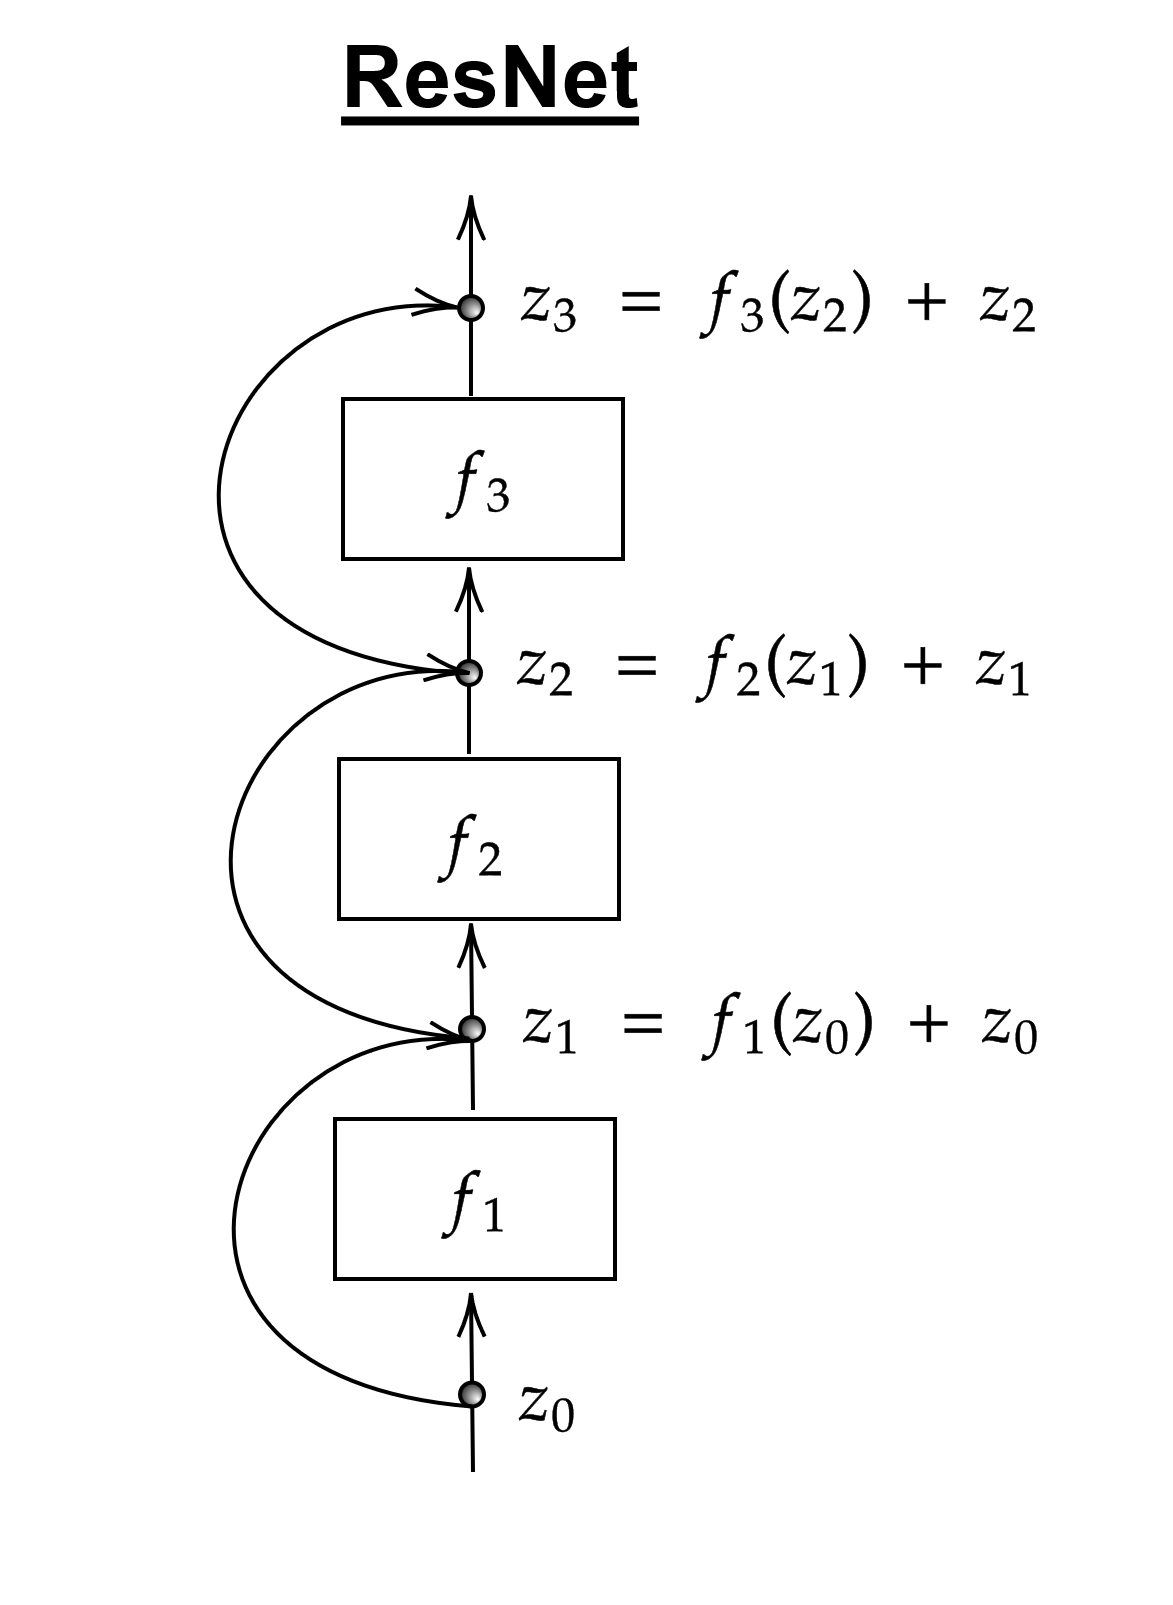
\includegraphics[scale=0.18]{resnet.png}
\caption{Example of residual neural network}
\label{exampleresnet}
\end{figure}

~

With these additional connections, we can avoid the problems of the \textit{vanishing gradient} and the \textit{exploding gradient} and thus have a better accuracy. 



Residual networks avoid the problem of vanishing gradient by introducing short paths which can carry a gradient over the entire extent of very deep networks. This is because adding the information from the previous layer will make these activations larger, so to some extent, they will prevent these activations from becoming exponentially small.

We can implement a simple ResNet to approximate the function
$$
h(x) = x^3 + 0.1x.
$$
To do that, we generate $10$ points between $-2.5$ and $2.5$. Their associated output comes from the function
$$
h(x) + \varepsilon,
$$
where $\varepsilon$ is a noise variable with mean $0$ and standard deviation $1$.

We train a ResNet with $3$ layers, the hidden one having $20$ neurons. After $1000$ iteration, we get the function given in Figure \ref{example_resnet}.

\begin{figure}[!h]
\center
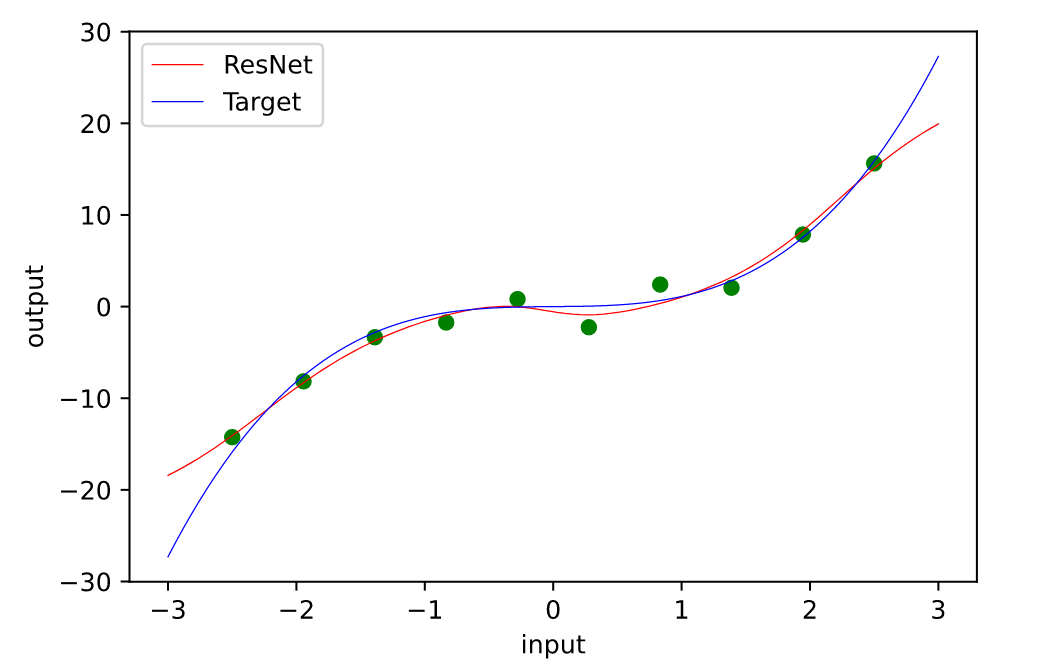
\includegraphics[scale=0.4]{ex_resnet.png}
\caption{Result of the training for the ResNet}
\label{example_resnet}
\end{figure}

The green points represent the data used for the training, the blue line is the function we want to approximate and the red line is the function represented by the ResNet. The out-of-sample error for the points used to trace the line is $4.6735477$.


\subsection{Implicit Layers}

There is two different ways to define a layer : \textit{explicitly} or \textit{implicitly} \cite{2}. When we define a layer explicitly, we specify the exact sequence of operations to do from the input to the output layer like in the example of the section \ref{exnn}. 

However, when we add some functionality to the layers, it can become complex to define them explicitly. Instead, we can define them implicitly: we specify the condition we want the layer's output to satisfy. 

An \textit{explicit layer} is defined by a function $f : \mathcal{X} \rightarrow \mathcal{Y}$. For an implicit layer, we give a condition that a function $g: \mathcal{X} \times \mathcal{Y} \rightarrow \mathbb{R}^n$ should satisfy. For example we can search for a $y$ such that $g(x,y) = 0$.

%\subsection{Implicit function theorem}
%
%Sometimes, variables can not be defined by a function but are rather defined by an equation. In this case, the \textit{implicit function theorem} can be used. It says that if a function $f$ is sufficiently regular in the neighborhood of a point, then there exists a function $\varphi$ at least as regular as $f$ such that locally, the graph of $f$ and the graph of $\varphi$ are the same.
%
%\begin{theorem}{\textbf{The implicit function theorem}}
%
%Let $f: \mathbb{R}^p \times \mathbb{R}^n \rightarrow \mathbb{R}^n$ be a function and $a_0 \in \mathbb{R}^p , z_0 \in \mathbb{R}^n$ two vectors such that :
%
%\begin{enumerate}
%\item $f(a_0,z_0) = 0$;
%\item $f$ is continuously differentiable with a non-singular Jacobian, i.e. its determinant is non zero, $\partial_z f(a_0,z_0) \in \mathbb{R}^{n \times n}$.
%\end{enumerate}
%Then there exist open sets $S_{a_0} \subset \mathbb{R}^p$ and $S_{z_0} \subset \mathbb{R}^n$ containing $a_0$ and $z_0$, respectively, and a unique continuous function $z*:S_{a_0} \rightarrow S_{z_0}$ such that:
%\begin{itemize}
%\item $z_0=z^*(a_0)$,
%\item $ \forall a \in S_{a_0}, f(a,z^*(a))=0$,
%\item $z^*$ is differentiable on $S_{a_0}$.
%\end{itemize}
%\end{theorem}
%
%We could use the theorem to compute the derivatives for the backpropagation, but in the following we will use a simpler derivation based on ResNet with the adjoint method.

\section{Neural ODE} \label{neuralode}

\subsection{Introduction}

In a residual neural network, the output for an input $x$ is a composition of functions. We want to extract all these individual layers to only have one "shared" layer.

A \textit{neural ODE network} (or ODE-Net) \cite{1,2,3,6} takes a simple layer as a building block. This “base layer” is going to specify the dynamics of an ODE.
ODE-Net enable us to replace layers of neural networks with a continuous-depth model. This means that we do not need to specify the number of layers beforehand.

Let us return to ResNets to give intuition behind this definition. We know that any output of the $k^{th}$ layer of a residual network can be computed with the function
\begin{equation*}
F(z_t, t; \theta) = f(z_t, t) + z_t
\end{equation*}
where $t = k - 1$.

Thus, in the ResNet, the output for the input $z_0 = x$ is a composition of the functions $F(z_t, t; \theta)$ where $\theta$ represents the parameters of the layers.


\begin{figure}
\center
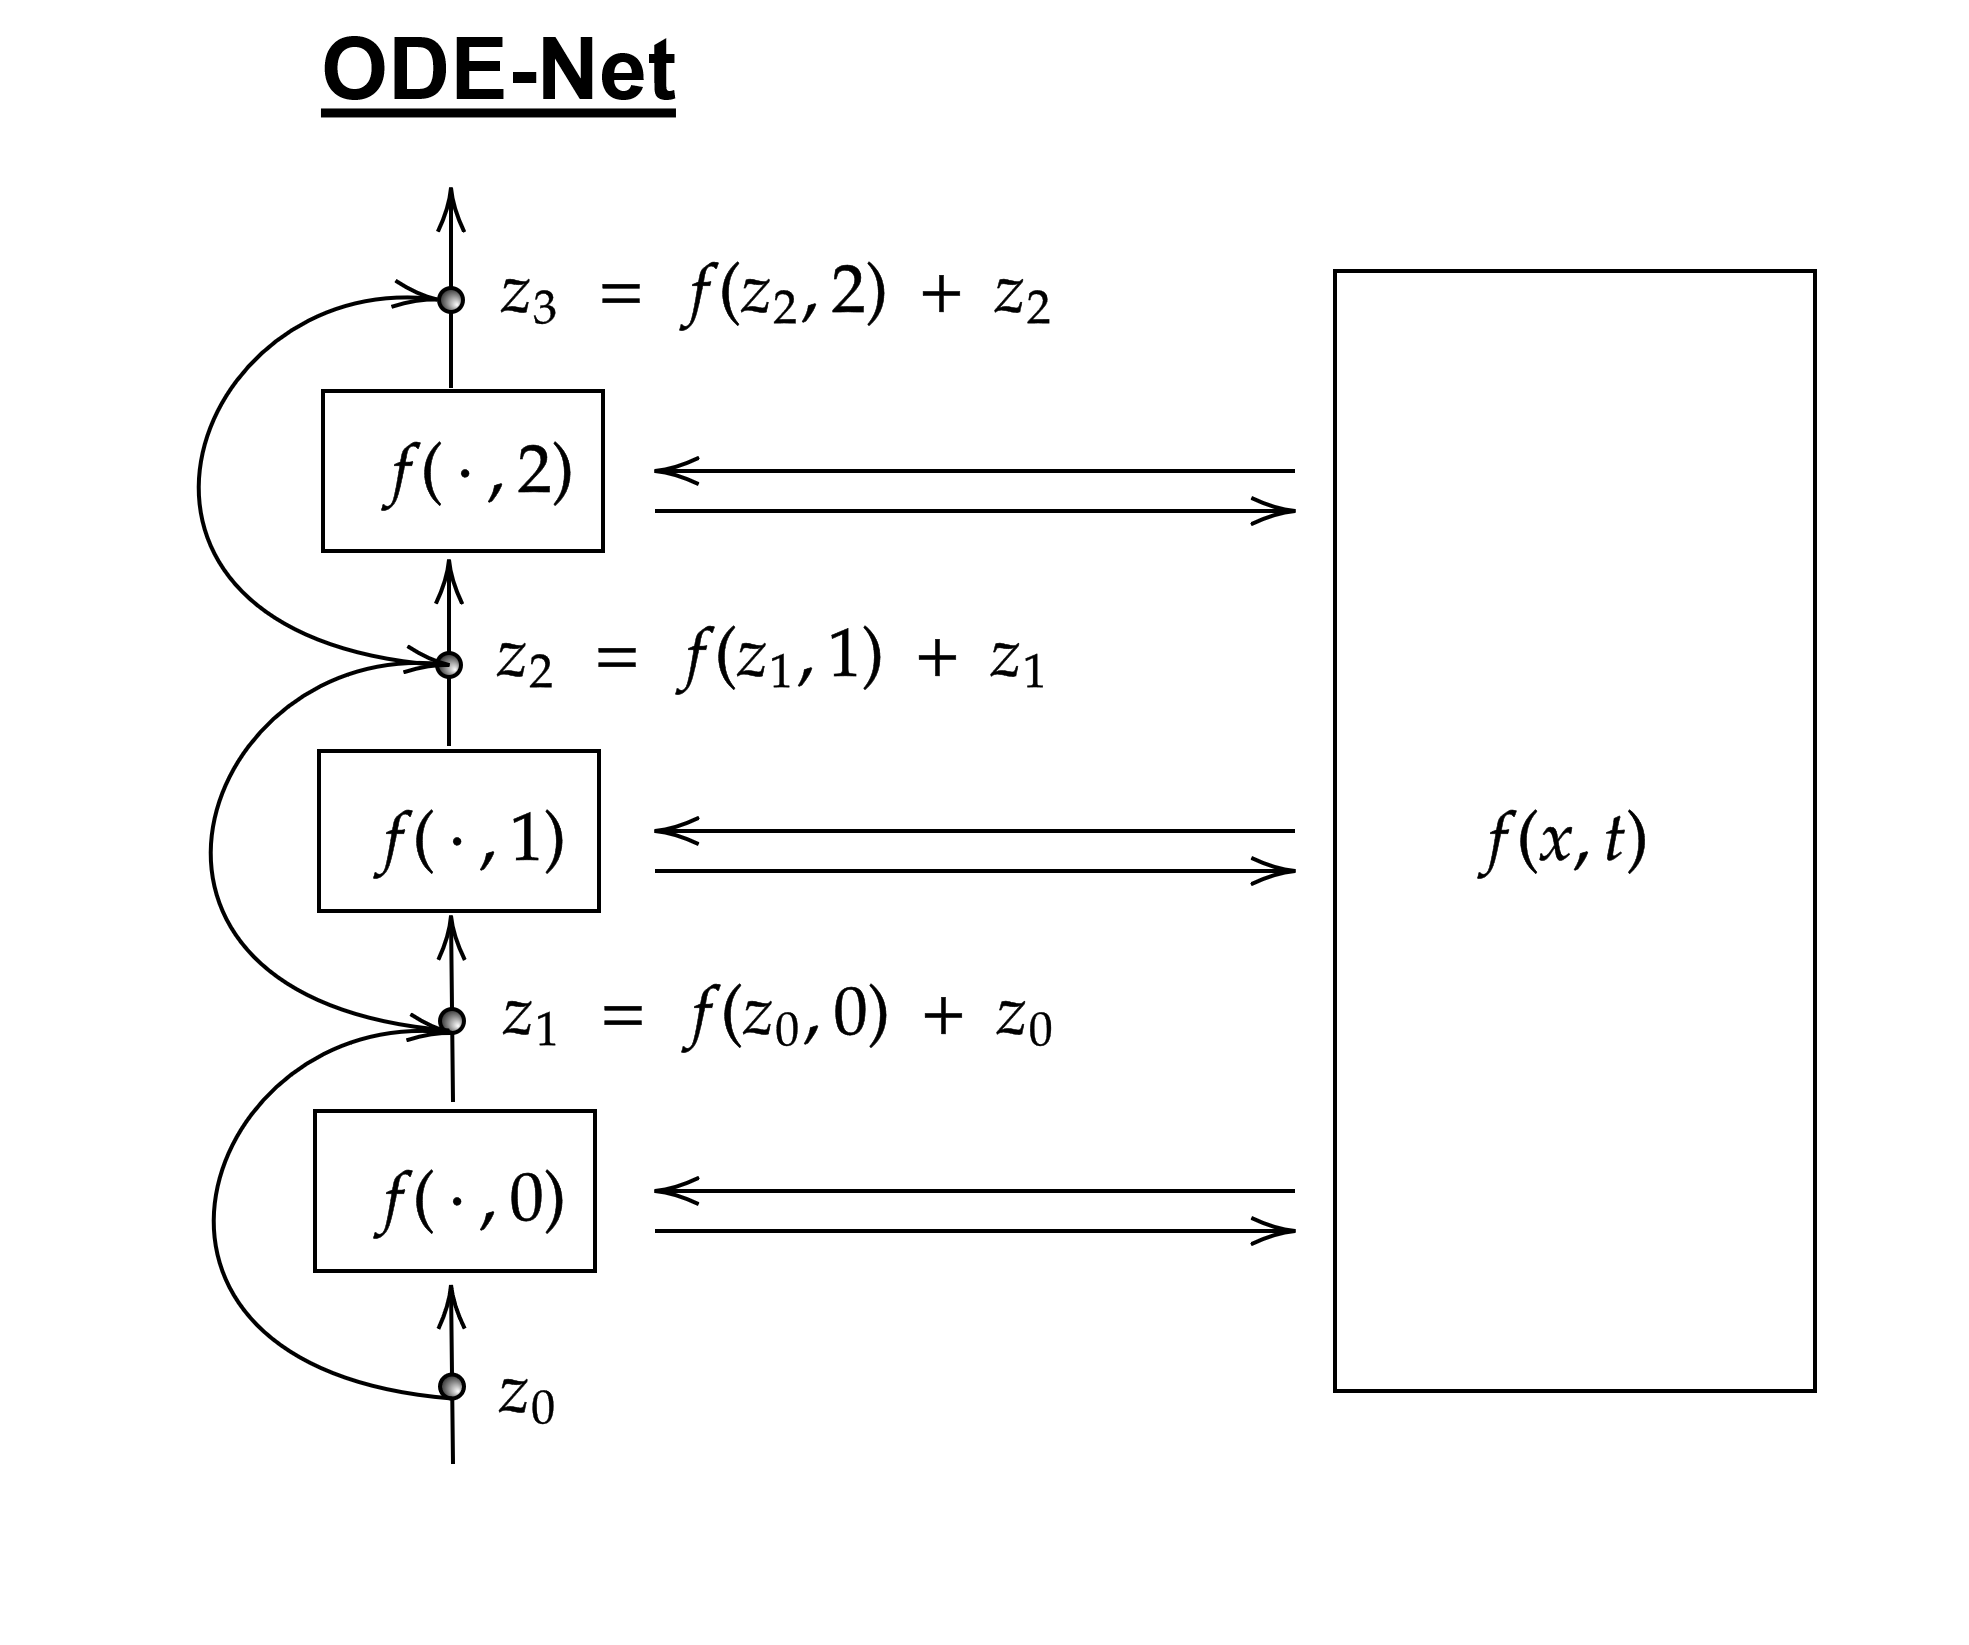
\includegraphics[scale=0.18]{ODENet.png}
\caption{Representation of an ODE-Net}
\end{figure}

We can then view $z$ as a function of $t$. For example,
\begin{equation*}
z(1) = f(x, 0) + x.
\end{equation*}
With that, we can write $F(z_t, t, \theta) = F(z(t), t, \theta)$. However, we need to give it the initial value of $z$, which is $z(t_0) = x$ (the input).

~

We saw that in ResNets, the outputs of each layer are the solutions of an ODE using Euler's method (cf Section \ref{euler}). The ODE from which it is a solution is $\frac{\partial z}{\partial t}(t) = f(z(t),t;\theta)$. But here we want to use a more precise method and then use a more complex ODE solver such as linear multistep methods. With what we've just shown, it is possible !

If we consider that the value given by $f(z(t), t, \theta)$ is the derivative of $z(t)$, we obtain the following Cauchy problem:
\begin{equation}
\label{cauchypb}
\begin{cases}
\frac{\partial z}{\partial t}(t) =  f(z(t), t; \theta) \\
z(t_0) =  x
\end{cases}
\end{equation}


\subsection{Forward pass}

The layer in an ODE-Net is implicit. The output $z(t_N)$ of an ODE-Net with the input $z(t_0)$ is defined by the Cauchy problem (\ref{cauchypb}). We see that the Cauchy problem depends on the parameters $z(t_0),t_0,t_N,\theta$.

But how do we solve this problem? We can simply use an ODE Solver with the parameters given above. In the case of the Euler method, the result is equivalent to a residual neural network, as we saw in Section \ref{rnn}.

To be able to use an ODE solver we have to make sure that the function satisfies the hypotheses in the theorem of existence and uniqueness (cf Section \ref{exiunique}). For example, if the activation function used in the network is ReLu, we can't apply the theorem since it is not differentiable at $0$.

\subsection{Backward pass: the Adjoint method}
Now that we know how to calculate the output of an ODE-Net, we need a method to find the optimal parameters that minimize the loss function.

In regular neural networks, we usually use the gradient descent. However in our case, it is more difficult because we used an ODE solver in the forward pass which is some sort of black box. This is why we are introducing the \textit{adjoint method} \cite{1}. This method computes the gradient by solving a second ODE backwards and is applicable to all ODE solvers.

Let $\mathcal{L} : \mathbb{R}^p \rightarrow \mathbb{R}$ be a loss function. To minimize this loss function $\mathcal{L}$, we need gradients with respect to the parameters $z(t_0),t_0,t_N,\theta$. To achieve that, we can determine how the gradient of the loss depends on the hidden state $z(t)$ for each $t$, which is
\begin{equation}
a(t)= \frac{\partial \mathcal{L}}{\partial z(t)}
\end{equation}

This quantity is called the \textit{adjoint}. We would like to determine its dynamics, so we need to compute its derivative with respect to $t$.

With a continuous hidden state, we can write the transformation after an $\varepsilon$ change in time as :
\begin{equation}
\label{zteps}
z(t+\varepsilon) = \int^{t+\varepsilon}_{t} f(z(t),t,\theta) dt + z(t)
\end{equation}
% car f(..) = d(z) et z(1) = z(0) + z(1) - z(0)
Let $ G : \varepsilon \mapsto z(t+\varepsilon)$. We can apply the Chain rule and we have 
\begin{equation*}
\frac{\partial \mathcal{L}}{\partial z(t)} = \frac{\partial \mathcal{L}}{\partial z(t+\varepsilon)} \frac{\partial z(t+\varepsilon)}{\partial z(t)}.
\end{equation*}
In other words 
\begin{equation}
\label{at}
a(t) = a(t+\varepsilon)\frac{\partial G(\varepsilon)}{\partial z(t)}
\end{equation}


We can now compute the derivative of $a(t)$ :
\begin{eqnarray*}
\frac{\partial a}{\partial t}(t) &=& \lim_{\varepsilon \rightarrow 0^+} \frac{a(t+\varepsilon) - a(t)}{\varepsilon} \text{ by definition of the derivative.}\\
&=& \lim_{\varepsilon \rightarrow 0^+} \frac{a(t+\varepsilon) - a(t+\varepsilon)\frac{\partial G(\varepsilon)}{\partial z(t)}}{\varepsilon} \text{ by (\ref{at}).}\\
&=& \lim_{\varepsilon \rightarrow 0^+} \frac{a(t+\varepsilon) - a(t+\varepsilon)\frac{\partial z(t) + \varepsilon f(z(t),t,\theta) + O(\varepsilon^2)}{\partial z(t)}}{\varepsilon}  \text{ by Taylor's development of G in 0.} \\
&=& \lim_{\varepsilon \rightarrow 0^+} \frac{a(t+\varepsilon) - a(t+\varepsilon)(\mathds{1} + \varepsilon \frac{\partial f(z(t),t,\theta)} {\partial z(t)}+ O(\varepsilon^2))}{\varepsilon}\\
&=& \lim_{\varepsilon \rightarrow 0^+} \frac{-\varepsilon a(t+\varepsilon) \frac{\partial f(z(t),t,\theta)} {\partial z(t)}+ O(\varepsilon^2)}{\varepsilon}\\
&=& \lim_{\varepsilon \rightarrow 0^+} - a(t+\varepsilon) \frac{\partial f(z(t),t,\theta)} {\partial z(t)}+ O(\varepsilon)\\
&=& -a(t)\frac{\partial f(z(t),t,\theta)} {\partial z(t)}
\end{eqnarray*}

We now have the dynamics of $a(t)$
\begin{equation}
\label{dynat}
\frac{\partial a(t)}{\partial t} = -a(t)\frac{\partial f(z(t),t,\theta)} {\partial z(t)}
\end{equation}
 
As we are searching for $ a(t_0) = \frac{\partial L}{\partial z(t_0)}$, we need to solve an ODE for the adjoint backwards in time because the value for $a(t_N)$ is already known. The constraint on the last time point, which is simply the gradient of the loss with respect to $z(t_N)$, 
\begin{equation*}
a(t_N) = \frac{\partial \mathcal{L}}{\partial z(t_N)},
\end{equation*}
has to be specified to the ODE solver. Then, the gradients with respect to the hidden state can be calculated at any time, including the initial value. We have 

\begin{eqnarray*}
a(t_0) &=& a(t_N) + \int^{t_0}_{t_N} \frac{\partial a(t)}{\partial t} dt \text{ by the fondamental theorem of calculus}\\
	   &=& a(t_N) - \int^{t_0}_{t_N} a(t) \frac{\partial f(z(t),t,\theta)} {\partial z(t)} dt \text{ par (\ref{dynat})}.
\end{eqnarray*}
If we want to compute the gradient with respect to the parameters $\theta$, we have to evaluate another integral, which depends on both $z(t)$ and $a(t)$,
\begin{equation}
\label{devtheta}
\frac{\partial L}{\partial \theta} = - \int^{t_0}_{t_N} a(t) \frac{\partial f(z(t),t,\theta)} {\partial \theta} dt.
\end{equation}
To avoid computing each ODE on its own, we can do all of them at the same time. To do that we can generalize the ODE to
\begin{eqnarray*}
\frac{\partial}{\partial t} \begin{bmatrix}
							z \\ \theta \\ t
							\end{bmatrix} (t) 
= f_{aug}([z(t),\theta ,t]) := \begin{bmatrix}
							f([z(t),\theta ,t]) \\ 0 \\ 1
							\end{bmatrix}, \\
a_{aug} (t) := \begin{bmatrix}
			a \\ a_{\theta} \\ a_t
			\end{bmatrix} (t) , \ 
a(t) = \frac{\partial \mathcal{L}}{\partial z(t)}, \ 
a_\theta (t) = \frac{\partial \mathcal{L}}{\partial \theta (t)}, \ 
a_t(t) := \frac{\partial \mathcal{L}}{\partial t(t)}.
\end{eqnarray*}

The jacobian of $f$ has the form
\begin{equation*}
\frac{\partial f_{aug}}{\partial [z(t),\theta,t]}([z(t),\theta,t]) = \begin{bmatrix}
\frac{\partial f}{\partial z} & \frac{\partial f}{\partial \theta} & \frac{\partial f}{\partial t} \\
\textbf{0} & \textbf{0} & \textbf{0} \\
\textbf{0} & \textbf{0} & \textbf{0}
\end{bmatrix}(t)
\end{equation*}

where each \textbf{0} is a matrix of zeros with the corresponding dimensions.

We can inject $a_{aug}$ in (\ref{dynat}) and we get
\begin{eqnarray*}
\frac{\partial a_{aug}(t)}{\partial t} 
&=& - [a(t) \ a_\theta (t) \ a_t (t)]\frac{\partial f_{aug}}{\partial [ z(t),\theta , t]}([z(t),\theta , t]) \\
&=& -\Big[a\frac{\partial f}{\partial z} \ a\frac{\partial f}{\partial \theta} \ a\frac{\partial  f}{\partial t}\Big] (t).
\end{eqnarray*}


We can see that the first component, $-a(t)\frac{\partial f(z(t),t,\theta)}{\partial z(t)}$, is the adjoint differential equation that we calculated previously in (\ref{dynat}). The total gradient with respect to the parameters is given by integrating the second component, $-a(t)\frac{\partial f(z(t),t,\theta)}{\partial \theta(t)}$ over the full interval and by setting $a_\theta (t_N) = \textbf{0}$. We obtain 
\begin{equation*}
\frac{\partial \mathcal{L}}{\partial \theta} = a_\theta (t_0) = - \int_{t_N}^{t_0} a(t) \frac{\partial f(z(t),t,\theta)}{\partial \theta} dt.
\end{equation*}

%sans a(tn) = 0 , on a a(tn) - integrale non ?

We can also get gradients with respect to $t_0$ and $t_N$ by integrating the last component, $-a(t)\frac{\partial f(z(t),t,\theta)}{\partial t(t)}$, and by the Chain rule respectively. We have
\begin{eqnarray*}
\frac{\partial \mathcal{L}}{\partial t_0} &=& a_t(t_0) = a_t(t_N) - \int_{t_N}^{t_0} a(t) \frac{\partial f(z(t),t,\theta)}{\partial t} dt ; \\
\frac{\partial \mathcal{L}}{\partial t_N} &=& \frac{\partial \mathcal{L}}{\partial z(t_N)} \frac{\partial z(t_N)}{\partial t_N} = a(t_N)f(z(t_N),t_N,\theta).
\end{eqnarray*}
With this generalized method, we have gradients for all possible inputs to a Cauchy problem solver. In the development above, we assumed that the loss function $L$ depends only on the last time point $t_N$. If function $L$ depends also on intermediate time points $t_1, t_2, \dots , t_{N-1}$, we can repeat the adjoint step for each of the intervals $[t_{N-1}, t_N ],[t_{N-2}, t_{N-1}], \dots , [t_0,t_1]$ in the backward order and sum up the obtained gradients.

%\subsection{Example}
%
%ODE-Net are very useful but they can't approximate any function. 
%For example, the simple function $f(x) = x^2$ can't be approximated by an ODE-Net because it's not a bijective function.
%
%As we can see in figure \ref{x2}, the network have a problem with negative numbers: the lines can't cross and that causes the negative values to be mapped to $0$.
%\begin{figure}[!h]
%\center
%\label{x2}
%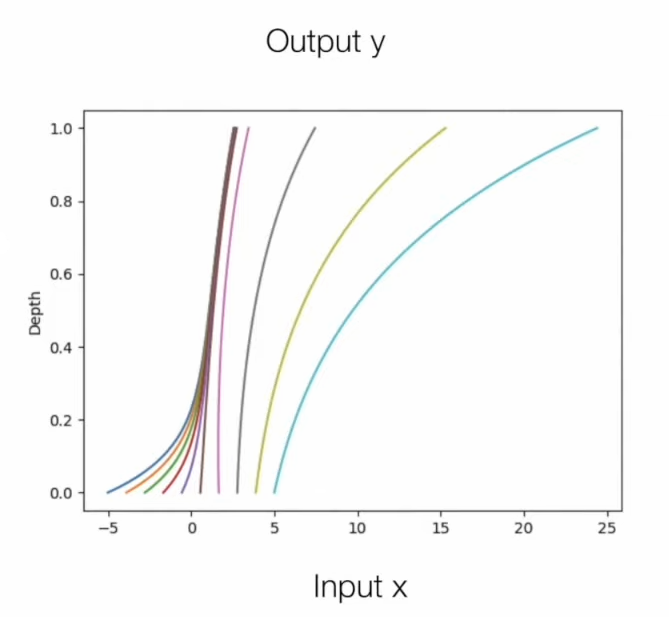
\includegraphics[scale=0.45]{x2graphe.png}
%\caption{Evolution of the output from the ODE-Net w.r.t. the depth.}
%\end{figure}
%
%On the other hand, ResNets have no problem approximating this type of function.
%
%\begin{figure}[!h]
%\center
%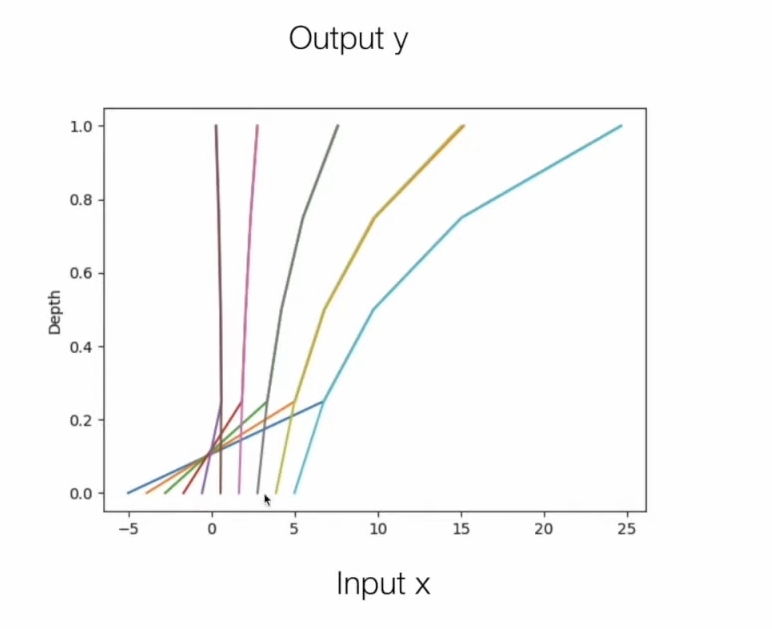
\includegraphics[scale=0.45]{x2gres.png}
%\caption{Evolution of the output from the ResNet w.r.t. the depth}
%\end{figure}

We can represent this process with the Figure \ref{process}. As we can see, during the forward pass, the loss function is evaluated a each time to be able to determine the smallest error.
\begin{figure}[!h]
\center
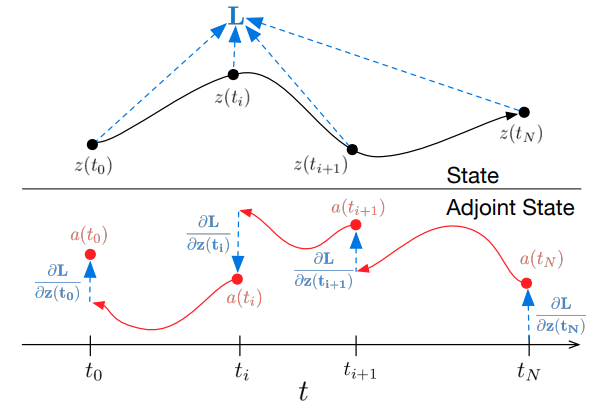
\includegraphics[scale=0.7]{fig2.png}
\caption{Graphical representation of the forward and backward pass for the ODE-Net. The figure has been taken from the paper \cite{1}.}
\label{process}
\end{figure}

\subsection{Simple Example}

Let's reuse the example for ResNets. We have the function 
$$
h(x) = x^3 + 0.1x
$$
that we wish to approximate.We use the same training data as for the ResNet.

The dynamics of the ODE-Net is specified by a layer of size $20$. After $1000$ iteration, we get the function given in Figure \ref{example_odenet}.

\begin{figure}[!h]
\center
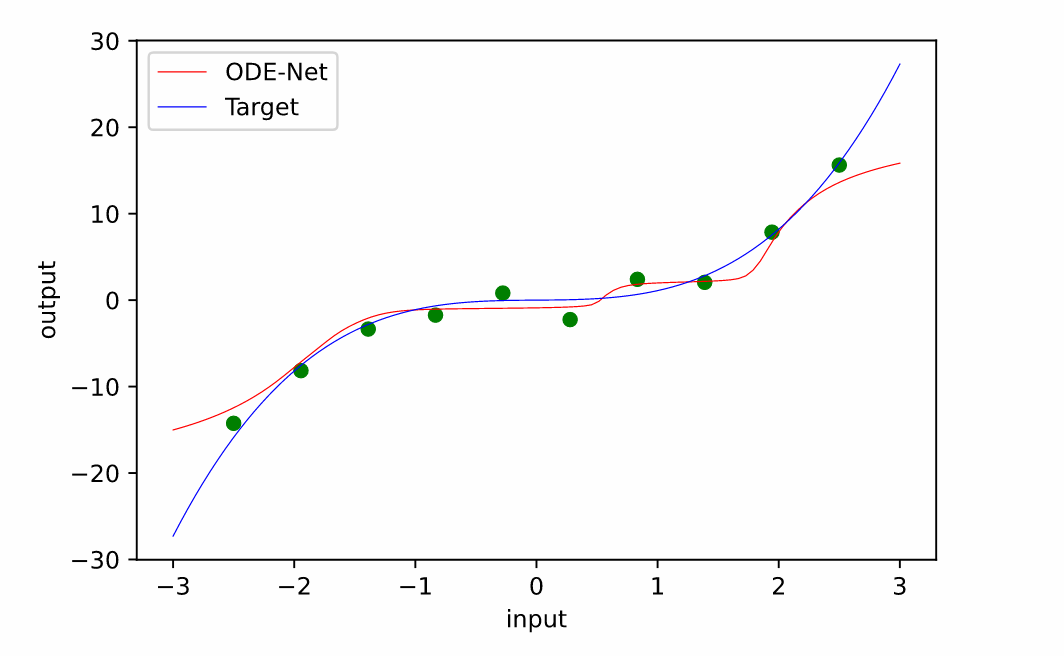
\includegraphics[scale=0.4]{ex_odenet.png}
\caption{Result of the training for the ODE-Net}
\label{example_odenet}
\end{figure}

The green points represent the data used for the training, the blue line is the function we want to approximate and the red line is the function represented by the ODE-Net.

We can compare these results with those we had for the ResNet, we can see that the ResNets is slightly better with these parameters. The comparison graph is in the Figure \ref{comparaison}.
\begin{figure}[!h]
\center
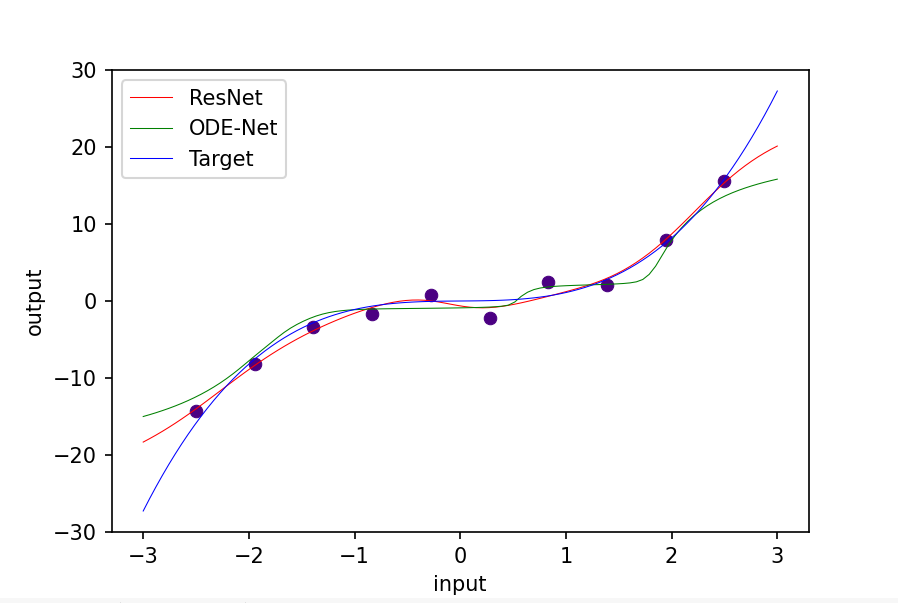
\includegraphics[scale=0.45]{comparaison.png}
\caption{Comparison of ResNet and ODE-Net}
\label{comparaison}
\end{figure}

\newpage

\subsection{Advantages and disadvantages of ODE-Nets}

\subsubsection*{Advantages}
\begin{itemize}
\item \textit{Continuous time series predictions}

The biggest advantage of ODE-Nets is that they have more accurate results for time series predictions. Regular neural network have discrete layers, which means they expect the intervals for these time series data sets to be fixed whereas ODE-Net have a continuous layer which means we can evaluate the hidden states at every point $t$ in time. Therefore, regular neural networks are bad at predicting output for time series data that is irregular.

\item \textit{ODE solvers}

We can use ordinary differential equations solvers instead of gradient descent. These solvers have more than a hundred years of theory behind them which is a great advantage against gradient descent.

\item \textit{Robustness} \cite{4}

After experimenting, it was proved that ODE-Net are very robust against perturbed data compared to regular neural network. Two experiments were conducted: in the first one they trained an ODE-Net and a convolutional neural network\footnote{A neural network that is usually good with images.} on real images without perturbations. They tested these models on the original images and the ODE-Net outperformed the CNN. In the second experiment, they trained these networks on the original and perturbed images. Again, the ODE-Net was much better.

\item \textit{Constant memory cost}

Lastly, there's a constant memory cost, instead of increasing the cost linearly with each layer in a regular network. 
In ODE-Net, we know the state at every time $t$. Because of that, we can always reconstruct the entire trajectory of an ODE forwards and backwards in time only by knowing this point. This means that ODE-Nets can be trained with a memory cost constant in the number of evaluations of $f$.
There is a trade-off between memory cost and computational time: ResNets are faster but use more memory and ODE-Net are slower but use less memory.
\end{itemize}

\subsubsection*{Disadvantages}
\begin{itemize}
\item \textit{Slower training time}

ODE-Net have a slower training time. Indeed, during training, the dynamics we want to learn tend to become expensive to solve since the network becomes deeper. However, regular neural networks can be evaluated with a fixed amount of computation, and are typically faster to train. In this case, we don't have to choose an error tolerance for a solver.

There is then a trade-off between accuracy and computational time: if we choose a small error tolerance, then the computational time be bigger.

\item \textit{More Hyperparameters}

In ODE-Nets we need to choose a solver and its error tolerance, which induces more choices to find the parameters which works better.

\item \textit{Restriction on activation functions}

To ensure that the ODE has a solution we have to make sure the dynamics are uniformly continuous Lipschitz (q.v. Theorem \ref{exiunique}). This is why we mostly use $tanh$ as an activation function.
\end{itemize}

\section{Annex}\label{annex}

\begin{definition}
Let   $$\begin{array}{rclc}
f: & \mathbb{R}^n & \rightarrow &  \mathbb{R}^m \\
&x = (x_1, \dots, x_n) & \mapsto & f(x_1, \dots, x_n)
\end{array}$$ be a function.

The \textit{partial derivative} of $f$ with respect to the variable $x_i$ is denoted by
$$
\frac{\partial f}{\partial x_i} :\mathbb{R}^n \rightarrow \mathbb{R}^m.
$$

For $a\in \mathbb{R}^n$, the partial derivative of $f$ with respect to $x_i$, if it exists, is defined as
$$
\frac{\partial f}{\partial x_i}(a) = \lim_{h\rightarrow0}\frac{f(a_1,\dots , a_{i-1}, a_i + h, a_{i+1}, \dots a_n) - f(a_1,\dots, a_i,\dots, a_n)}{h}.
$$
\end{definition}

\begin{definition}
Let $f: \mathbb{R}^n \rightarrow \mathbb{R}^m$ be a function and $a\in \mathbb{R}^n$.
We can write the \textit{first-order Taylor's development} for $f$ at $x$ as :
$$
f(x + a) = f(x) + a . \partial f(x) + O(\| a\|^2).
$$
\end{definition}

\begin{definition}
Le $f: \mathbb{R}^n \rightarrow \mathbb{R}$ be function, $n\geq 2$. Then $f$ is \textit{convex} if and only if
$$
\forall 0\leq t \leq 1, \forall x_1,x_2\in \mathbb{R}^n, \ \ \ f(tx_1 + (1-t)x_2) \leq tf(x_1) + (1-t)f(x_2)
$$
\end{definition}

\begin{definition}
If $f$ and $g$ are differentiable functions, then the \textit{chain rule} expresses the derivative of their composite $f \circ g$ in terms of the derivatives of $f$ and $g$ and the product of functions as follows:
$$
\frac{\partial f \circ g}{\partial x} = \Big(\frac{\partial f}{\partial x} \circ g\Big)\frac{\partial g}{\partial x}
$$
\end{definition}

\begin{theorem} \label{thmconvgd}
Si $f : \mathbb{R}^d \to \mathbb{R}$ est une fonction L-Lipschitzienne convexe et si $x^* = argmin_x f(x)$, alors l'algorithme de descente du gradient avec la taille de pas $\eta \leqslant \frac{1}{L}$ satisfait
$$
f(x_{k}) \leqslant f(x^*) + \frac{\|x_0 - x^* \|_2}{2\eta k} .
$$
\end{theorem}

\section{References}

\nocite{*}
\bibliography{biblio}
\bibliographystyle{plain}




\end{document}